\documentclass{poly}
\usepackage{main}

\title{Chapitre 4 : Généralités sur les fonctions}
\author{Seconde 3}
\date{}

\begin{document}
\maketitle

\section{Définitions}
\begin{definition}
Une \textbf{fonction} est un objet mathématique capable d'associer un \textbf{unique} résultat à tout objet d'un ensemble appelé \textbf{ensemble de définition}. 
\end{definition}
\begin{example}
On définit plusieurs fonctions dont l'ensemble de définition est \emph{l'ensemble des élèves de la seconde 3} :
\begin{itemize}
\item $f$ est la fonction qui à un élève de la seconde 3 associe sa date d'anniversaire.
\item $g$ est la fonction qui à un élève de la seconde 3 associe sa couleur préférée.
\item $h$ est la fonction qui à un élève de la seconde 3 associe l'initiale d'un des membres de sa famille. \textbf{(Attention ! A-t-on vraiment défini une fonction ici ?)}
\item $p$ est la fonction qui à un élève de la seconde 3 associe 
\item $q$ est la fonction qui à un élève de la seconde 3 associe 
\end{itemize}
\end{example}
\begin{remark}
On s'intéresse majoritairement en mathématiques aux fonctions numériques. Les ensembles de définitions sont des ensembles de nombres, et le résultat renvoyé par les fonctions est toujours un nombre réel.
\end{remark}
\begin{definition}
Une \textbf{fonction numérique à valeurs réelles} est une fonction $f$ définie de la manière suivante :
\begin{equation*}
\function{f}{I}{\R}{x}{f(x)}
\end{equation*}
avec $I$ son \textbf{ensemble de définition}.
\end{definition}
\begin{remark}
\hfill
\begin{itemize}
\item La plupart du temps, on aura $I = \R$, $I$ est un intervalle ou $I$ est une réunion d'intervalles.
\item On aura toujours $\R$ à droite de la flèche du haut : on dit que \textbf{l'ensemble d'arrivée} est $\R$.
\item La flèche du bas se lit de la manière suivante : au nombre $x$, on renvoie le nombre $f(x)$
\end{itemize}
\end{remark}
\begin{definition}
Soit $\function{f}{I}{\R}{x}{f(x)}$ et $a \in I$. On pose $b$ vérifiant l'égalité
\begin{equation*}
b = f(a)\,.
\end{equation*}
Alors, 
\begin{itemize}
\item $a$ est \textbf{un antécédent} de $b$ par la fonction $f$.
\item $b$ est \textbf{l'image} de $a$ par la fonction $f$.
\end{itemize}
\end{definition}
\begin{example}
Soit $\function{f}{\R}{\R}{x}{2x+1}$.
\begin{alphaquestions}
\item Donner l'image de $3$ par $f$ : 
\item Donner un antécédent de $7$ par $f$ : 
\end{alphaquestions}
\end{example}
\newpage
\section{Courbe représentative}

\begin{definition}
Soit $f$ une fonction définie sur un ensemble de définition $I$. On se place sur un reprère orthonormé. Alors, la \textbf{courbe représentative de $f$}, notée $\mathcal{C}_f$, est l'ensemble des points du repère de coordonnées $(x;y)$ vérifiant
\begin{equation*}
y = f(x)
\end{equation*}
\end{definition}
\begin{remark}
Chaque point de la courbe de coordonnées $(x;y)$ représente une association entre antécédent et image : 
\begin{itemize}
\item l'abscisse $x$ du point joue le rôle de l'antécédent; 
\item l'ordonnée $y$ du point joue le rôle de l'image.
\end{itemize}
\end{remark}
\begin{example}
Soit $f$ une fonction dont la courbe représentative est donnée sur le repère orthonormé suivant. Donner l'image de $3$ par $f$: 
\begin{center}
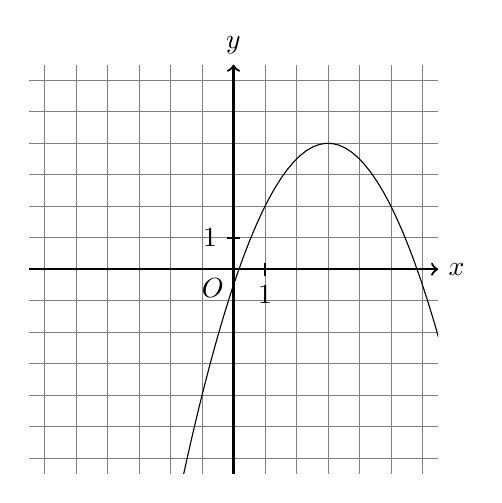
\begin{tikzpicture}[scale=0.8]
\draw[help lines] (-3.25,-3.25) grid[step=0.5] (3.25,3.25);
\draw[thick, ->] (-3.25,0) -- (3.25,0) node[right] {$x$};
\draw[thick, ->] (0,-3.25) -- (0,3.25) node[above] {$y$};
\draw (0,0) node[below left] {$O$};
\draw[thick] (0.5,0.1) -- (0.5,-0.1) node[below] {$1$};
\draw[thick] (0.1,0.5) -- (-0.1,0.5) node[left] {$1$};
\clip (-3.25,-3.25) rectangle (3.25,3.25);
\draw[samples=100] plot (\x,{-(\x-1.5)*(\x - 1.5) + 2});
\end{tikzpicture}
\end{center}
\end{example}

\subsection{Calcul des antécédents de $f$}
Pour chercher un antécédent (ou tous les antécédents) d'un nombre $a$ par $f$, on trace une droite horizontale d'équation $y = a$ :
\begin{example}
\hfill
\begin{center}
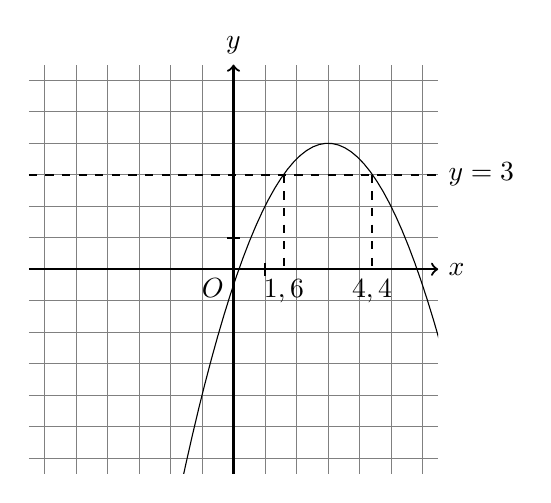
\begin{tikzpicture}[scale=0.8]
\draw[help lines] (-3.25,-3.25) grid[step=0.5] (3.25,3.25);
\draw[thick, ->] (-3.25,0) -- (3.25,0) node[right] {$x$};
\draw[thick, ->] (0,-3.25) -- (0,3.25) node[above] {$y$};
\draw (0,0) node[below left] {$O$};
\draw[thick] (0.5,0.1) -- (0.5,-0.1);
\draw[thick] (0.1,0.5) -- (-0.1,0.5);
\draw[thick,dashed] (-3.25,1.5) -- (3.25,1.5) node[right] {$y = 3$};
\draw[thick,dashed] (0.8,1.5) -- (0.8,0) node[below] {$1,6$};
\draw[thick,dashed] (2.2,1.5) -- (2.2,0) node[below] {$4,4$};
\clip (-3.25,-3.25) rectangle (3.25,3.25);
\draw[samples=100] plot (\x,{-(\x-1.5)*(\x - 1.5) + 2});
\end{tikzpicture}
\end{center}
On a résolu ici l'équation $f(x) = 3$ : l'ensemble $\mathcal{S}$ des solutions est donné par $\mathcal{S} = \{1,6; 4,4\}$.
\end{example}

\newpage

\subsection{Résolution d'inéquation $f(x) \geq a$}
Dans ce cas, on cherche les zones où la courbe est \textbf{au-dessus} de la droite horizontale d'équation $y = a$.
\begin{example}
\hfill
\begin{center}
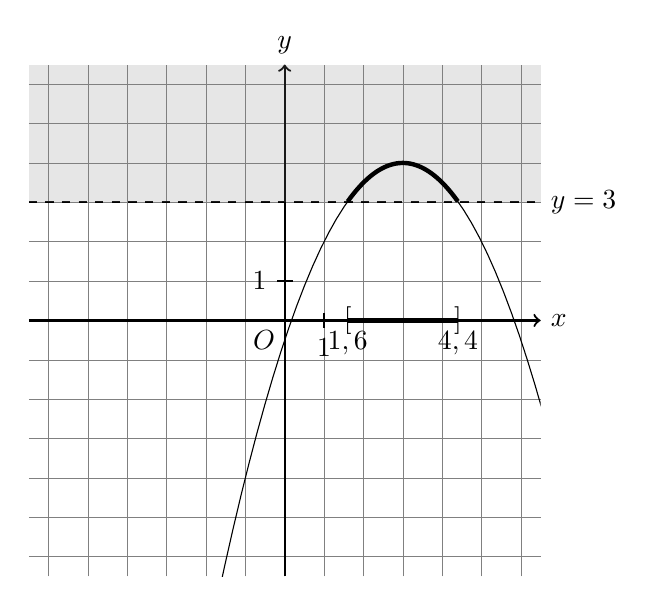
\begin{tikzpicture}
\draw[help lines] (-3.25,-3.25) grid[step=0.5] (3.25,3.25);
\draw[thick, ->] (-3.25,0) -- (3.25,0) node[right] {$x$};
\draw[thick, ->] (0,-3.25) -- (0,3.25) node[above] {$y$};
\draw (0,0) node[below left] {$O$};
\draw[thick] (0.5,0.1) -- (0.5,-0.1) node[below] {$1$};
\draw[thick] (0.1,0.5) -- (-0.1,0.5) node[left] {$1$};
\draw[thick,dashed] (-3.25,1.5) -- (3.25,1.5) node[right] {$y = 3$};
\fill[color=gray,opacity=0.2] (-3.25,1.5) rectangle (3.25,3.25);
\draw[ultra thick] (0.8,0) node {$[$} node[below] {$1,6$} -- (2.2,0) node {$]$} node[below] {$4,4$};
\clip (-3.25,-3.25) rectangle (3.25,3.25);
\draw[samples=100] plot (\x,{-(\x-1.5)*(\x - 1.5) + 2});
\draw[samples=100,domain=0.8:2.2,ultra thick] plot (\x,{-(\x-1.5)*(\x - 1.5) + 2});
\end{tikzpicture}
\end{center}
Ici, on a résolu l'inéquation $f(x) \geq 3$ : l'ensemble des solutions $\mathcal{S}$ de cette inéquation est donné par l'intervalle $[1,6;4,4]$.
\end{example}
\begin{tcolorbox}
\begin{remark}
\hfill
\begin{itemize}
\item Le sens des crochets est toujours dépendant des cas d'égalités.
\item La même méthode marche pour $f(x) > a$; $f(x) \leq a$ et $f(x) < a$.
\item Si la courbe est au-dessus de la droite à plusieurs endroit, alors on \og joint \fg les différents intervalles-solutions à l'aide du symbole $\cup$ (qui se lit \textbf{\og union \fg}). Par exemple, $[0;1] \cup ]4,5;9]$ est une union d'intervalles.
\end{itemize}
\end{remark}
\end{tcolorbox}

\newpage

\subsection{Résolution d'équation $f(x)=g(x)$}
Cette information est donnée par les points d'intersection des courbes représentatives des fonctions $f$ et $g$
\begin{example}
\hfill
\begin{center}
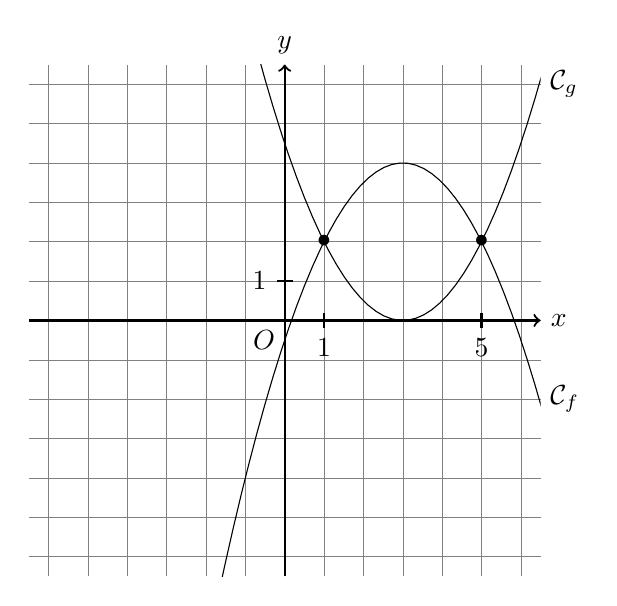
\begin{tikzpicture}
\draw[help lines] (-3.25,-3.25) grid[step=0.5] (3.25,3.25);
\draw[thick, ->] (-3.25,0) -- (3.25,0) node[right] {$x$};
\draw[thick, ->] (0,-3.25) -- (0,3.25) node[above] {$y$};
\draw (0,0) node[below left] {$O$};
\draw[thick] (0.5,0.1) -- (0.5,-0.1) node[below] {$1$};
\draw[thick] (0.1,0.5) -- (-0.1,0.5) node[left] {$1$};
\draw (0.5,1) node {$\bullet$};
\draw (2.5,1) node {$\bullet$};
\draw[thick] (2.5,0.1) -- (2.5,-0.1) node[below] {$5$};
\draw (3.25,-1) node[right] {$\mathcal{C}_f$};
\draw (3.25,3) node[right] {$\mathcal{C}_g$};
\clip (-3.25,-3.25) rectangle (3.25,3.25);
\draw[samples=100] plot (\x,{-(\x-1.5)*(\x - 1.5) + 2});
\draw[samples=100] plot (\x,{(\x-1.5)*(\x - 1.5)});
\end{tikzpicture}
\end{center}
L'ensemble des solutions de $f(x)=g(x)$ est donné par $\mathcal{S} = \{1;5\}$.
\end{example}
\subsection{Résolution d'inéquation $f(x) < g(x)$}
Cette information est donnée par la position relative entre les deux courbes représentatives.
\begin{example}
\hfill
\begin{center}
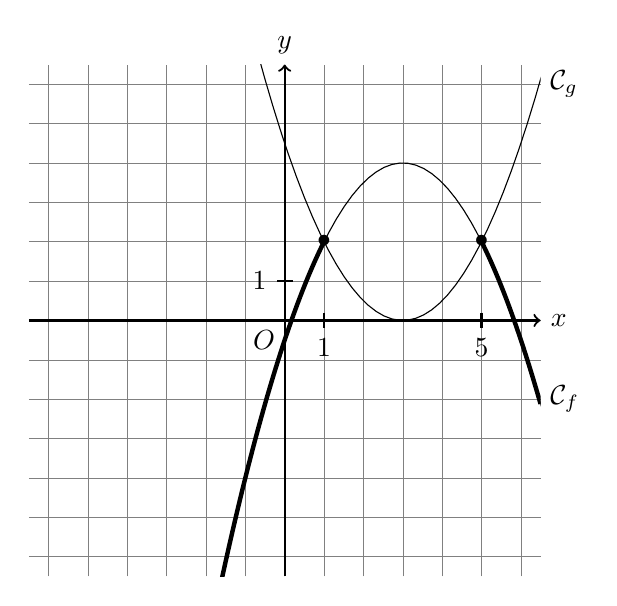
\begin{tikzpicture}
\draw[help lines] (-3.25,-3.25) grid[step=0.5] (3.25,3.25);
\draw[thick, ->] (-3.25,0) -- (3.25,0) node[right] {$x$};
\draw[thick, ->] (0,-3.25) -- (0,3.25) node[above] {$y$};
\draw (0,0) node[below left] {$O$};
\draw[thick] (0.5,0.1) -- (0.5,-0.1) node[below] {$1$};
\draw[thick] (0.1,0.5) -- (-0.1,0.5) node[left] {$1$};
\draw (0.5,1) node {$\bullet$};
\draw (2.5,1) node {$\bullet$};
\draw[thick] (2.5,0.1) -- (2.5,-0.1) node[below] {$5$};
\draw (3.25,-1) node[right] {$\mathcal{C}_f$};
\draw (3.25,3) node[right] {$\mathcal{C}_g$};
\clip (-3.25,-3.25) rectangle (3.25,3.25);
\draw[samples=100] plot (\x,{-(\x-1.5)*(\x - 1.5) + 2});
\draw[samples=100] plot (\x,{(\x-1.5)*(\x - 1.5)});
\draw[samples=100, domain=-3.25:0.5, ultra thick] plot (\x,{-(\x-1.5)*(\x - 1.5) + 2});
\draw[samples=100, domain=2.5:3.25, ultra thick] plot (\x,{-(\x-1.5)*(\x - 1.5) + 2});
\end{tikzpicture}
\end{center}
L'ensemble $\mathcal{S}$ des solutions de l'inéquation $f(x)<g(x)$ est donné par la réunion d'intervalles $]-\infty;1[\cup]5;+\infty[$.
\end{example}

\end{document}